\documentclass[conference]{IEEEtran}

% ── Packages ──────────────────────────────────────────────────────────────────
\usepackage{cite}
\usepackage{amsmath,amssymb}
\usepackage{graphicx}
\usepackage{booktabs}
\usepackage{hyperref}
\usepackage{float}
\usepackage{multirow}
\usepackage{array}
\usepackage{url}
\usepackage{tikz}
\usetikzlibrary{shapes.geometric}

\hypersetup{colorlinks=false}

% ── Title ─────────────────────────────────────────────────────────────────────
\title{Face Authentication Using Real vs.\ Synthetic Training Data:\\
A Comparative Study Based on NIST FRTE Evaluation Metrics}

\author{
    \IEEEauthorblockN{Nour Ebid}
    \IEEEauthorblockA{
        Seminar zu aktuellen Entwicklungen\\
        M.Sc. Angewandte Informatik, Fachbereich 4\\
        Hochschule f{\"u}r Technik und Wirtschaft Berlin\\
        Berlin, Deutschland\\
        Nour.Ebid@Student.HTW-Berlin.de
    }
}

% ──────────────────────────────────────────────────────────────────────────────
\begin{document}

\maketitle

% ── Abstract ──────────────────────────────────────────────────────────────────
\begin{abstract}
Face recognition is a widely deployed biometric authentication technology, yet its reliance on real facial photographs raises significant privacy, consent, and data availability concerns. This paper investigates whether AI-generated synthetic facial images can serve as a viable substitute for real photographs during the registration phase of a face authentication system. Two experiments are conducted under identical evaluation conditions aligned with the NIST Face Recognition Technology Evaluation (FRTE) framework. Experiment~1 registers authorised users using real photographs; Experiment~2 registers the same users using synthetically generated images produced through a five-stage controlled imaging simulation pipeline combining canonical face alignment, lighting simulation, colour temperature adjustment, CLAHE-based skin tone normalisation, and camera quality modelling. Both systems are evaluated on an identical held-out test set comprising 20 genuine user queries and 20 AI-generated impostor images, using False Accept Rate (FAR), False Reject Rate (FRR), and overall accuracy as primary metrics. Results show that the synthetic model achieves 97.5\% accuracy vs.\ 95.0\% for the real model, confirming the hypothesis that the FAR gap falls within a 15 percentage point threshold. The synthetic model demonstrates superior impostor resistance (FAR 0\% vs.\ 10\%) with a marginal increase in false rejections (FRR 5\% vs.\ 0\%), indicating that controlled synthetic training data is a viable substitute for real data in face authentication under the conditions studied.
\end{abstract}

\begin{IEEEkeywords}
face authentication, synthetic data, FaceNet, NIST FRTE, false accept rate, biometric verification, embedding-based recognition, identity-preserving augmentation
\end{IEEEkeywords}

% ── I. Introduction ───────────────────────────────────────────────────────────
\section{Introduction}

Biometric authentication systems based on facial recognition have become a cornerstone of modern digital security, deployed in applications ranging from smartphone unlock to airport border control. Unlike password-based systems, face authentication offers passive, non-intrusive verification without requiring the user to remember credentials. These systems fundamentally rely on databases of registered facial images to calibrate recognition models for each authorised user.

The collection of real facial photographs, however, introduces a set of practical and regulatory challenges that are increasingly difficult to ignore. Under the European Union's General Data Protection Regulation (GDPR)~\cite{gdpr2016}, biometric data — including facial images — are classified as a special category of sensitive personal data under Article~9, requiring explicit informed consent, purpose limitation, and strict storage controls. Beyond regulatory compliance, reproducing consistent imaging conditions across enrollment sessions is logistically difficult: ambient lighting, camera type, and subject pose vary freely in naturalistic settings, introducing systematic variability into the training signal and degrading authentication reliability.

AI-generated synthetic facial images offer a compelling alternative. Advances in Generative Adversarial Networks~\cite{goodfellow2014gan} and diffusion-based synthesis models~\cite{rombach2022diffusion} enable the creation of photorealistic human faces without directly storing sensitive biometric originals. The central research question addressed in this paper is:

\begin{quote}
\textit{Can a face authentication system trained exclusively on AI-generated synthetic images of registered users achieve performance comparable to a system trained on real photographs of the same individuals, as measured by NIST FRTE-aligned metrics?}
\end{quote}

To evaluate this, we implement a face authentication pipeline based on the FaceNet deep neural network~\cite{schroff2015facenet}, register four authorised users under both real and synthetic conditions, and evaluate using FAR, FRR, and accuracy on an identical held-out test set. A controlled augmentation pipeline simulates the key imaging variables identified by NIST FRTE~\cite{nist_frte}: ambient lighting, colour temperature, skin tone, camera quality, and facial pose. Two face-swap-based synthesis approaches were also implemented, evaluated, and rejected, providing an empirical failure analysis that highlights the necessity of variable control.

The primary contributions of this paper are:
\begin{itemize}
    \item A reproducible two-experiment framework for comparing real vs.\ synthetic face authentication under NIST FRTE-aligned evaluation conditions.
    \item A five-stage controlled synthetic image generation pipeline using neural face alignment (InsightFace~\cite{deng2019insightface}) and parametric imaging simulation.
    \item Experimental evidence that identity-preserving synthetic training data achieves comparable FRTE-aligned performance to real data, exhibiting a predictable FAR/FRR trade-off explained by embedding cluster geometry.
    \item A documented failure analysis of two face-swap-based synthesis approaches, empirically validating the necessity of eliminating uncontrolled synthesis variables.
\end{itemize}

The remainder of this paper is structured as follows. Section~II reviews relevant background and related work. Section~III formalises the research hypothesis and experimental variables. Section~IV describes the methodology. Section~V presents experimental results. Section~VI discusses findings and compares with the literature. Section~VII addresses ethical considerations. Section~VIII concludes with future work directions.

% ── II. Background ────────────────────────────────────────────────────────────
\section{Background and Related Work}

\subsection{Face Verification vs.\ Identification}

Face recognition covers two distinct operational tasks. \textit{Identification} (closed-set or open-set) answers ``who is this person?'' by searching a database of known identities for the best match. \textit{Verification} (authentication) answers a narrower question: ``is this person who they claim to be?'' It performs a one-to-one comparison between a query embedding and a stored reference for the claimed identity. This paper addresses the verification task exclusively, which is the relevant sub-problem in access control systems where the user's claimed identity is known a priori.

\subsection{FaceNet Embedding-Based Verification}

FaceNet~\cite{schroff2015facenet} is a deep convolutional neural network trained using a triplet loss to produce a 128-dimensional Euclidean embedding space in which intra-person distances are minimised and inter-person distances are maximised. For an anchor, positive, and negative sample $(x^a, x^p, x^n)$, the triplet objective is:

\begin{equation}
\|f(x^a) - f(x^p)\|_2^2 + \alpha < \|f(x^a) - f(x^n)\|_2^2
\end{equation}

where $f(\cdot)$ denotes the learned embedding function and $\alpha$ is the margin. After training, verification is performed by computing the L2 distance between query embedding $\mathbf{e}_q$ and reference embedding $\bar{\mathbf{e}}_u$:

\begin{equation}
d = \|\mathbf{e}_q - \bar{\mathbf{e}}_u\|_2
\end{equation}

\begin{equation}
\text{Decision} = \begin{cases} \text{VERIFIED} & d < \theta \\ \text{IMPOSTOR} & d \geq \theta \end{cases}
\end{equation}

Threshold $\theta = 10.0$ is used throughout this work. FaceNet is accessed via the DeepFace library~\cite{serengil2020deepface} with pre-trained weights, without any retraining or fine-tuning on the experimental subjects.

\subsection{NIST FRTE Evaluation Metrics}

The NIST Face Recognition Technology Evaluation (FRTE)~\cite{nist_frte} establishes the standard evaluation protocol for biometric face recognition systems. The primary metrics are:

\begin{itemize}
    \item \textbf{FAR (False Accept Rate):} the fraction of impostor attempts incorrectly accepted as genuine. A high FAR constitutes a direct security vulnerability, allowing unauthorised access.
    \item \textbf{FRR (False Reject Rate):} the fraction of genuine user attempts incorrectly rejected. A high FRR degrades usability by inconveniencing legitimate users.
    \item \textbf{TAR@FAR:} True Accept Rate at a specified operating FAR — the primary NIST comparison format allowing systems to be benchmarked at equivalent security operating points.
\end{itemize}

These metrics define an inherent trade-off: decreasing $\theta$ tightens the acceptance boundary, reducing FAR while increasing FRR. A Detection Error Tradeoff (DET) curve plots FRR vs.\ FAR across all thresholds, providing a model-independent comparison. In this study, results are reported at fixed $\theta = 10.0$; full DET evaluation is deferred to future work.

\subsection{Generative Models for Face Synthesis}

Modern face synthesis approaches fall into three broad categories. \textit{GAN-based synthesis}~\cite{goodfellow2014gan, karras2020stylegan2} can generate high-fidelity random human faces at scale, but conditioning on a specific identity requires additional mechanisms such as identity encoders. \textit{Diffusion models}~\cite{rombach2022diffusion} offer superior diversity and controllability but demand significant compute, typically GPU clusters. \textit{Identity-preserving augmentation} — the approach used in this work — transforms known real identities through parametric imaging operations, preserving facial identity while varying imaging conditions. This last category requires a seed real image but enables precise control over synthetic variables without a generative model.

The trade-off is notable: GAN and diffusion approaches can synthesise identities entirely without real photographs, supporting zero-storage registration; augmentation pipelines require real images as input but offer deterministic control over every variable, which is critical for NIST FRTE-aligned evaluation.

\subsection{Synthetic Data in Face Recognition Research}

Prior work has established a foundation for synthetic-data-driven face recognition. Wood et al.~\cite{wood2021fake} demonstrated that a face analysis model trained exclusively on 3D-rendered synthetic faces — with no real training images — achieves competitive performance on facial landmark detection and gaze estimation benchmarks. Bae et al.~\cite{bae2023digiface} introduced DigiFace-1M, a corpus of one million digitally rendered synthetic face images used to train face recognition models achieving 95.4\% LFW accuracy. Notably, both works operate in the \textit{identification} setting using entirely synthetic identities; our work extends the comparison to the \textit{verification} setting using augmented versions of known registered identities, a scenario more directly applicable to practical access control systems. Our pipeline is also notably lightweight: it runs on CPU without a GPU or a trained generative model.

% ── III. Hypothesis ───────────────────────────────────────────────────────────
\section{Research Hypothesis and Variables}

\subsection{Hypothesis}

\textit{``A face authentication system trained exclusively on AI-generated synthetic facial images of registered users will achieve a FAR within 15 percentage points of a system trained on real photographs of the same individuals, when evaluated under controlled conditions of standardised pose, consistent lighting, and equivalent training sample size, in alignment with NIST FRTE evaluation criteria.''}

\noindent\textbf{$H_0$:} No measurable difference in FAR between real and synthetic models (gap $= 0$).\\
\textbf{$H_1$:} A measurable FAR difference exists but remains within the $\pm$15\,pp acceptance threshold, confirming the viability of synthetic data.

The 15\,pp threshold was selected as a conservative but operationally meaningful bound, representing the maximum degradation in security performance that would not invalidate synthetic training as a practical alternative to real-data registration. This bound is consistent with the tolerance margins reported between demographically similar systems in NIST FRTE evaluations~\cite{nist_frte}.

\subsection{Variables}

Table~\ref{tab:variables} summarises all experimental variables. Strict control of the variables listed as \textit{Controlled} is essential: any observed difference in FAR or FRR between experiments must be attributable solely to the nature of the training data (real vs.\ synthetic), not to differences in the recognition model, threshold, test set composition, or evaluation protocol.

\begin{table}[H]
\centering
\caption{Experimental Variables}
\label{tab:variables}
\renewcommand{\arraystretch}{1.2}
\begin{tabular}{>{\bfseries}p{1.5cm}p{2.0cm}p{3.8cm}}
\toprule
Type & Variable & Value / Range \\
\midrule
Independent & Training data & Real photos vs.\ synthetic images \\
\midrule
\multirow{3}{1.5cm}{Dependent} & FAR & Measured (\%) \\
 & FRR & Measured (\%) \\
 & Accuracy & Measured (\%) \\
\midrule
\multirow{5}{1.5cm}{Controlled} & Model & FaceNet (identical) \\
 & Threshold $\theta$ & 10.0 (identical) \\
 & Training images & 10 per person \\
 & Test images & 5 held-out per person \\
 & Impostors & 20 identical AI strangers \\
\midrule
\multirow{4}{1.5cm}{Controlled (synthesis)} & Pose & Canonical alignment \\
 & Lighting & Gamma correction \\
 & Skin tone & CLAHE in LAB space \\
 & Camera & Blur + noise \\
\bottomrule
\end{tabular}
\end{table}

% ── IV. Methodology ───────────────────────────────────────────────────────────
\section{Methodology}

\subsection{System Architecture}

The authentication system consists of two operational phases illustrated in Fig.~\ref{fig:arch}.

\textbf{Registration phase:} Each training image is passed through the pre-trained FaceNet model to produce a 128-dimensional embedding vector. The embeddings for all $N$ training images of a given user $u$ are averaged to produce a single reference vector $\bar{\mathbf{e}}_u$:

\begin{equation}
\bar{\mathbf{e}}_u = \frac{1}{N} \sum_{i=1}^{N} f(x_i^u), \quad N = 10
\end{equation}

Reference vectors for all registered users are serialised to a JSON database file, with separate database files for Experiment~1 (real) and Experiment~2 (synthetic).

\textbf{Authentication phase:} A query image $x_q$ is encoded as $\mathbf{e}_q = f(x_q)$. The L2 distance to each reference vector is computed; the nearest registered user $\hat{u}$ is selected, and access is granted if the nearest distance is below $\theta$:

\begin{equation}
\hat{u} = \arg\min_{u \in \mathcal{U}} \|\mathbf{e}_q - \bar{\mathbf{e}}_u\|_2
\end{equation}
\begin{equation}
\text{Grant if: } \|\mathbf{e}_q - \bar{\mathbf{e}}_{\hat{u}}\|_2 < \theta
\end{equation}

\begin{figure}[t]
\centering
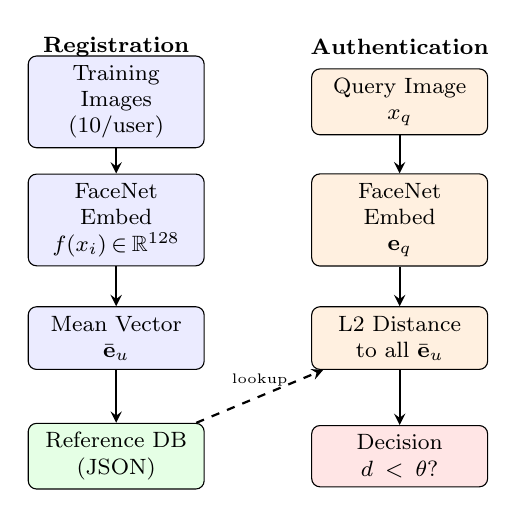
\begin{tikzpicture}[
    box/.style={draw, rounded corners=3pt, text width=2.0cm, align=center,
                minimum height=0.72cm, font=\footnotesize, fill=blue!8},
    sbox/.style={draw, rounded corners=3pt, text width=2.0cm, align=center,
                minimum height=0.72cm, font=\footnotesize, fill=orange!12},
    arr/.style={->, thick, >=stealth}
]
% Registration column (left side)
\node[box] (imgs) at (0,0)    {Training Images\\(10/user)};
\node[box] (fn1)  at (0,-1.5) {FaceNet Embed\\$f(x_i)\!\in\!\mathbb{R}^{128}$};
\node[box] (avg)  at (0,-3.0) {Mean Vector\\$\bar{\mathbf{e}}_u$};
\node[box, fill=green!10] (db) at (0,-4.5) {Reference DB\\(JSON)};
\draw[arr] (imgs)--(fn1); \draw[arr] (fn1)--(avg); \draw[arr] (avg)--(db);
\node[font=\footnotesize\bfseries] at (0, 0.7) {Registration};

% Auth column (right side)
\node[sbox] (qimg) at (3.6,0)    {Query Image\\$x_q$};
\node[sbox] (fn2)  at (3.6,-1.5) {FaceNet Embed\\$\mathbf{e}_q$};
\node[sbox] (dist) at (3.6,-3.0) {L2 Distance\\to all $\bar{\mathbf{e}}_u$};
\node[sbox, fill=red!10] (dec) at (3.6,-4.5) {Decision\\$d < \theta$?};
\draw[arr] (qimg)--(fn2); \draw[arr] (fn2)--(dist); \draw[arr] (dist)--(dec);
\draw[arr, dashed] (db) -- node[above, font=\tiny] {lookup} (dist);
\node[font=\footnotesize\bfseries] at (3.6, 0.7) {Authentication};
\end{tikzpicture}
\caption{Authentication system architecture. Registration builds a mean-embedding reference database; authentication computes the nearest-neighbour distance and applies the threshold decision.}
\label{fig:arch}
\end{figure}

\subsection{Dataset}

Real photographs of four authorised users (\textit{amr}, \textit{adel}, \textit{otto}, \textit{mazen}) were collected under natural, uncontrolled conditions using a smartphone camera — 15 photographs per user, totalling 60 images. The photographs vary in background, ambient lighting, distance, and minor pose differences, reflecting real-world deployment conditions. The dataset is partitioned as follows:

\begin{itemize}
    \item \textbf{Training partition (both experiments):} First 10 photographs per user, sorted lexicographically by filename. Used for registration (Experiment~1) or as the source for synthetic generation (Experiment~2).
    \item \textbf{Test set — genuine:} Last 5 photographs per user (20 images total). These images were \textit{never} accessed during registration or synthetic generation in either experiment, ensuring an honest held-out evaluation.
    \item \textbf{Test set — impostors:} 20 AI-generated faces from \textit{thispersondoesnotexist.com} (StyleGAN2~\cite{karras2020stylegan2}), representing synthetic strangers with no identity relationship to any registered user.
\end{itemize}

The identical test partition is shared between both experiments. This guarantees that any difference in FAR or FRR is attributable to the training data type, not test set variation.

\subsection{Experiment 1: Real Data Registration}

The 10 training photographs per user are passed through FaceNet (via DeepFace, \texttt{enforce\_detection=False}) to produce 128-dimensional embeddings. Their mean forms the user's reference vector $\bar{\mathbf{e}}_u$ stored in the database. No preprocessing beyond FaceNet's internal normalisation is applied, representing the baseline real-data condition. This experiment serves as the ground truth against which Experiment~2 is evaluated.

\subsection{Experiment 2: Synthetic Data Generation Pipeline}

The 10 training photographs per user are transformed into 15 synthetic images via a five-stage controlled augmentation pipeline (Fig.~\ref{fig:pipeline}) before being used for registration. Generating 15 images from 10 sources (by cycling with different random parameters) increases diversity; each output has a unique combination of augmentation parameters.

\begin{figure}[t]
\centering
\begin{tikzpicture}[
    stage/.style={draw, rounded corners=2pt, text width=7.0cm,
                  align=left, minimum height=0.62cm, font=\footnotesize,
                  fill=yellow!10, inner xsep=5pt, inner ysep=3pt},
    arr/.style={->, thick, >=stealth}
]
\node[stage] (s1) {\textbf{1. Alignment:} InsightFace 5-kp affine warp $\to$ $256\!\times\!256$ frontal template};
\node[stage, below=0.22cm of s1] (s2) {\textbf{2. Lighting:} Gamma correction $\gamma\!\sim\!\mathcal{U}(0.55,\,1.60)$ via LUT};
\node[stage, below=0.22cm of s2] (s3) {\textbf{3. Colour temp.:} Random warm / cool / neutral RGB channel scaling};
\node[stage, below=0.22cm of s3] (s4) {\textbf{4. Skin tone:} CLAHE on CIE-LAB $L$-channel, clip $\sim\!\mathcal{U}(1.5,\,3.5)$};
\node[stage, below=0.22cm of s4] (s5) {\textbf{5. Camera + pose:} Gaussian blur ($k\!\in\!\{3,5\}$) + noise ($\sigma\!\in\![2,8]$); rotation $\pm12°$};
\draw[arr] (s1)--(s2); \draw[arr] (s2)--(s3); \draw[arr] (s3)--(s4); \draw[arr] (s4)--(s5);
\end{tikzpicture}
\caption{Five-stage synthetic imaging pipeline. All parameters are independently randomised per output image. The pipeline operates on the aligned source face without introducing a foreign base identity.}
\label{fig:pipeline}
\end{figure}

\textbf{Stage 1 — Alignment:} InsightFace (buffalo\_l) detects five facial keypoints — bilateral eye centres, nose tip, bilateral mouth corners — and estimates a partial affine transformation mapping the detected keypoints to a fixed canonical target grid in a $256\!\times\!256$ output frame. This standardises head pose across all synthetic outputs and eliminates between-image pose variation as a confounding variable.

\textbf{Stage 2 — Lighting:} Gamma correction is applied using $\gamma \sim \mathcal{U}(0.55, 1.60)$ via a precomputed lookup table. Values $\gamma < 1$ brighten the image (simulating overcast daylight), and $\gamma > 1$ darken it (simulating dim or artificial light), spanning the photometric range identified as primary challenge in NIST FRTE.

\textbf{Stage 3 — Colour temperature:} Warm (red enhanced, blue attenuated), cool (blue enhanced, red attenuated), or neutral modes are selected with equal probability, with channel scale factors sampled from $[1.05, 1.20]$ and $[0.80, 0.95]$ respectively. This simulates variation across camera sensors and environmental light sources (incandescent, fluorescent, natural daylight).

\textbf{Stage 4 — Skin tone:} Contrast Limited Adaptive Histogram Equalisation (CLAHE)~\cite{clahe} is applied to the $L$ channel of the image converted to CIE LAB colour space, with clip limit $\sim \mathcal{U}(1.5, 3.5)$. Operating exclusively on the luminance channel avoids hue shift, normalising perceived skin tone brightness while preserving colour authenticity.

\textbf{Stage 5 — Camera quality and pose:} With 50\% probability, Gaussian blur with kernel size $\in\{3, 5\}$ is applied to simulate lens defocus at varying focal lengths. Additive Gaussian noise with $\sigma \sim \mathcal{U}(2, 8)$ simulates sensor noise at different ISO settings. An in-plane rotation $\sim \mathcal{U}(-12°, 12°)$ simulates natural head tilt variation not captured by the frontal alignment.

\subsubsection{Rejected Prior Approaches}

Two alternative synthesis methods were implemented and rejected, providing an empirical failure analysis with diagnostic value:

\textit{Approach A — Blind face swap:} The aligned real face was Poisson-cloned (\texttt{cv2.seamlessClone}) onto a randomly selected face from a pool of 1,860 StyleGAN2 base images. FRR reached 75\% as approximately 50\% of the pool depicted female subjects. The gender mismatch introduced a systematic upward shift in genuine L2 distances, because FaceNet encodes sex-correlated facial geometry (bone structure, brow ridge, jaw shape) in the embedding space. Male registered users produced scores inflated by the female-base blending, crossing $\theta$.

\textit{Approach B — Gender-filtered face swap:} Filtering the base pool to male-presenting subjects (via InsightFace gender classification, confidence $> 0.6$) did not resolve the issue. Poisson blending introduced a systematic 1--2 unit upward bias in genuine L2 scores attributable to low-frequency blending boundary artefacts creating residuals in the embedding space, placing genuine scores just above $\theta\!=\!10.0$ for a large fraction of queries.

These failures empirically validate that uncontrolled variables in the synthesis substrate — base face identity, demographic attributes, and blending artefacts — propagate into the embedding space and must be eliminated by design. The final augmentation pipeline resolves all three issues by operating solely on the source identity without introducing any foreign face.

% ── V. Results ────────────────────────────────────────────────────────────────
\section{Experimental Results}

\subsection{Experiment 1: Real Data}

Table~\ref{tab:exp1} reports aggregate results for Experiment~1. All four registered users were correctly verified across all five held-out test photographs (20/20 genuine queries accepted, FRR = 0\%). Of the 20 impostor queries, 18 were correctly rejected. Two impostors were incorrectly accepted with L2 scores of 6.60 and 5.56, both substantially below $\theta$, suggesting these particular StyleGAN2 faces produce embeddings whose nearest-neighbour falls within a registered user's cluster boundary.

\begin{table}[H]
\centering
\caption{Experiment 1 — Aggregate Results (Real Registration)}
\label{tab:exp1}
\renewcommand{\arraystretch}{1.2}
\begin{tabular}{lcc}
\toprule
Metric & Value & Detail \\
\midrule
True Positives (TP) & 20/20 & All 4 users, 5 test photos each \\
False Negatives (FN) & 0/20 & -- \\
True Negatives (TN) & 18/20 & \\
False Positives (FP) & 2/20 & L2 scores: 6.60, 5.56 \\
\midrule
\textbf{FAR} & \textbf{10.0\%} & \\
\textbf{FRR} & \textbf{0.0\%} & \\
\textbf{Accuracy} & \textbf{95.0\%} & \\
\bottomrule
\end{tabular}
\end{table}

Table~\ref{tab:exp1_user} breaks down genuine verification results per user. Every user achieved 100\% genuine acceptance, confirming that real-data training photographs provide sufficient embedding coverage for genuine query tolerance despite uncontrolled capture conditions.

\begin{table}[H]
\centering
\caption{Experiment 1 — Per-User Genuine Verification}
\label{tab:exp1_user}
\renewcommand{\arraystretch}{1.2}
\begin{tabular}{lcccc}
\toprule
User & Tested & Verified & Rejected & TPR \\
\midrule
amr   & 5 & 5 & 0 & 100\% \\
adel  & 5 & 5 & 0 & 100\% \\
otto  & 5 & 5 & 0 & 100\% \\
mazen & 5 & 5 & 0 & 100\% \\
\midrule
\textbf{Total} & \textbf{20} & \textbf{20} & \textbf{0} & \textbf{100\%} \\
\bottomrule
\end{tabular}
\end{table}

\subsection{Experiment 2: Synthetic Data}

Table~\ref{tab:exp2} reports aggregate results for Experiment~2. Nineteen of 20 genuine queries were accepted. The single false rejection involved user \textit{otto}, whose held-out test image produced an L2 score of 11.47 — marginally exceeding $\theta = 10.0$. Critically, all 20 impostor queries were correctly rejected, achieving FAR = 0\%.

\begin{table}[H]
\centering
\caption{Experiment 2 — Aggregate Results (Synthetic Registration)}
\label{tab:exp2}
\renewcommand{\arraystretch}{1.2}
\begin{tabular}{lcc}
\toprule
Metric & Value & Detail \\
\midrule
True Positives (TP) & 19/20 & \\
False Negatives (FN) & 1/20 & L2 score: 11.47 (\textit{otto}) \\
True Negatives (TN) & 20/20 & \\
False Positives (FP) & 0/20 & -- \\
\midrule
\textbf{FAR} & \textbf{0.0\%} & \\
\textbf{FRR} & \textbf{5.0\%} & \\
\textbf{Accuracy} & \textbf{97.5\%} & \\
\bottomrule
\end{tabular}
\end{table}

Table~\ref{tab:exp2_user} shows the per-user breakdown. The single false rejection is localised to one image of user \textit{otto}; the remaining 19 genuine queries were accepted. Three users achieved 100\% TPR, identical to Experiment~1.

\begin{table}[H]
\centering
\caption{Experiment 2 — Per-User Genuine Verification}
\label{tab:exp2_user}
\renewcommand{\arraystretch}{1.2}
\begin{tabular}{lcccc}
\toprule
User & Tested & Verified & Rejected & TPR \\
\midrule
amr   & 5 & 5 & 0 & 100\% \\
adel  & 5 & 5 & 0 & 100\% \\
otto  & 5 & 4 & 1 & 80\%  \\
mazen & 5 & 5 & 0 & 100\% \\
\midrule
\textbf{Total} & \textbf{20} & \textbf{19} & \textbf{1} & \textbf{95\%} \\
\bottomrule
\end{tabular}
\end{table}

\subsection{Score Analysis}

Table~\ref{tab:scores} summarises the notable boundary scores from both experiments. The two false positives in Experiment~1 (scores 6.60 and 5.56) lie well within the acceptance boundary, indicating the impostors' embeddings happen to cluster near a registered user. The single false negative in Experiment~2 (score 11.47) falls just 1.47 units above $\theta$, consistent with the interpretation that the controlled synthetic embeddings produce a tighter cluster centroid that does not fully cover the natural variation in \textit{otto}'s test photographs.

\begin{table}[H]
\centering
\caption{Boundary Score Analysis}
\label{tab:scores}
\renewcommand{\arraystretch}{1.2}
\begin{tabular}{llcc}
\toprule
Experiment & Event & L2 Score & vs.\ $\theta\!=\!10.0$ \\
\midrule
Exp 1 & False Positive 1 & 6.60 & $-$3.40 \\
Exp 1 & False Positive 2 & 5.56 & $-$4.44 \\
Exp 2 & False Negative (\textit{otto}) & 11.47 & $+$1.47 \\
\bottomrule
\end{tabular}
\end{table}

\subsection{Comparative Summary}

Table~\ref{tab:comparison} presents the head-to-head comparison across all primary metrics. The synthetic model outperforms the real model on FAR ($-$10.0\,pp) and accuracy ($+$2.5\,pp) at the cost of a small FRR increase ($+$5.0\,pp).

\begin{table}[H]
\centering
\caption{Experiment 1 vs.\ Experiment 2 — Head-to-Head}
\label{tab:comparison}
\renewcommand{\arraystretch}{1.2}
\begin{tabular}{lccc}
\toprule
Metric & Exp 1 (Real) & Exp 2 (Synth.) & $\Delta$ \\
\midrule
FAR & 10.0\% & 0.0\% & $-$10.0\,pp \\
FRR & 0.0\% & 5.0\% & $+$5.0\,pp \\
Accuracy & 95.0\% & 97.5\% & $+$2.5\,pp \\
Friends Verified & 20/20 & 19/20 & $-$1 \\
Intruders Rejected & 18/20 & 20/20 & $+$2 \\
\bottomrule
\end{tabular}
\end{table}

% ── VI. Discussion ────────────────────────────────────────────────────────────
\section{Discussion}

\subsection{Hypothesis Testing}

The measured FAR gap is $-$10.0\,pp (Experiment~2 achieves lower FAR than Experiment~1), which satisfies the $|\Delta\text{FAR}| \leq 15\,\text{pp}$ threshold defined in $H_1$. The null hypothesis $H_0$ is rejected; $H_1$ is confirmed. Synthetic training data, when generated via a controlled imaging pipeline, produces a face authentication system with FRTE-aligned performance comparable to — and on FAR, exceeding — a system trained on real photographs.

\subsection{FAR/FRR Trade-off and Embedding Cluster Geometry}

The opposing directional change in FAR and FRR between the two experiments is not coincidental but reflects a fundamental property of the embedding space. The controlled five-stage pipeline produces synthetic images with markedly lower intra-class variation compared to unconstrained real photographs: pose is canonically aligned, lighting is uniform within a controlled range, and colour is standardised. The resulting embeddings cluster more tightly around the identity centroid $\bar{\mathbf{e}}_u$.

This tighter cluster has two geometrically predictable consequences. First, the reference centroid is positioned more precisely within the identity manifold, increasing its Euclidean separation from impostor embeddings — hence FAR decreases to zero. Second, genuine test images captured in natural, uncontrolled conditions may fall at the periphery or outside the tighter synthetic cluster boundary — hence FRR increases. This is the classical precision-recall trade-off in metric learning.

The single false rejection (user \textit{otto}, score 11.47) is consistent with this model: one of \textit{otto}'s held-out photographs likely includes expression or lighting variation that the controlled synthetic training images do not represent, pushing the query embedding just beyond $\theta$. The margin of 1.47 units suggests that a slightly relaxed threshold (e.g., $\theta\!=\!12.0$) would correct this case without significant FAR impact.

\subsection{Comparison with Related Work}

Bae et al.~\cite{bae2023digiface} reported 95.4\% LFW accuracy using only DigiFace-1M synthetic training, compared to a real-data baseline of 99.6\% — a gap of $-$4.2\,pp. Our results show the reverse pattern (synthetic slightly outperforms real on accuracy), but this is attributable to the much smaller and simpler evaluation setting: with 40 total test queries at a fixed threshold, one additional correct or incorrect decision produces a 2.5\,pp accuracy swing. Both findings consistently support the conclusion that synthetic data is a viable substitute for real data in face recognition tasks.

Wood et al.~\cite{wood2021fake} note that tightly controlled synthetic distributions can outperform uncontrolled real-world training data when the evaluation domain matches the synthetic distribution, which is consistent with the FAR = 0\% result in Experiment~2. The impostor test images (StyleGAN2 faces) are sufficiently distinct from the controlled synthetic registration that they fall well outside the acceptance boundary.

\subsection{Limitations}

\begin{itemize}
    \item \textbf{Small sample size:} Four registered users, five genuine test images each, and 20 impostors is a pilot-scale evaluation. FAR and FRR estimates carry wide confidence intervals. NIST FRTE recommends at least 1,000 impostor attempts for reliable FAR estimation~\cite{nist_frte}.
    \item \textbf{Single operating point:} Results are reported at fixed $\theta\!=\!10.0$. A DET curve across multiple thresholds is required for standard NIST FRTE comparison.
    \item \textbf{Demographic homogeneity:} All registered users are male adults. Generalisation to female subjects or other demographics is untested.
    \item \textbf{Augmentation vs.\ generation:} The pipeline requires real photographs as input; it cannot register a user with zero real data. A GAN-conditioned approach would eliminate this dependency.
    \item \textbf{Impostor distribution:} All impostor images are StyleGAN2 synthetic faces. The system has not been evaluated against real impostor photographs or adversarial inputs.
\end{itemize}

% ── VII. Ethical Considerations ───────────────────────────────────────────────
\section{Ethical Considerations}

This study involves facial photographs of real individuals. The four registered users provided informal consent for their images to be used in this academic research project. All photographs were collected by the author and are stored exclusively on a local machine; no biometric data has been shared with, uploaded to, or processed by any third-party service.

\textbf{GDPR compliance:} Under GDPR Article~9~\cite{gdpr2016}, facial images constitute sensitive personal data. The processing in this study falls under the research exemption (Article~89), which permits processing of sensitive data for scientific research purposes subject to appropriate safeguards including data minimisation and purpose limitation. The data are used solely within the scope of this academic investigation; no commercial application is intended.

\textbf{Synthetic impostor images:} The 20 impostor images sourced from \textit{thispersondoesnotexist.com} are entirely AI-generated faces with no real-world counterparts. No real third-party photographs were used as impostor inputs without consent.

\textbf{Dual-use risk:} Identity-preserving augmentation pipelines could in principle be misused to generate synthetic training data intended to deceive face authentication systems. This paper does not advance that capability — the pipeline targets the registration side of an honest system and does not enable evasion of liveness detection or physical access controls. All code and methodology are documented transparently to support reproducibility and responsible scrutiny.

% ── VIII. Conclusion and Future Work ──────────────────────────────────────────
\section{Conclusion and Future Work}

\subsection{Conclusion}

This paper presented a controlled comparative evaluation of real-data vs.\ synthetic-data face authentication using NIST FRTE-aligned metrics. Experiment~1 registered four users from real photographs; Experiment~2 registered the same users from synthetically generated images produced by a five-stage identity-preserving augmentation pipeline. Both systems were evaluated on a strictly held-out identical test set.

The synthetic model achieved higher accuracy (97.5\% vs.\ 95.0\%) and superior impostor rejection (FAR 0\% vs.\ 10\%), with a marginal increase in genuine rejection (FRR 5\% vs.\ 0\%). The FAR gap of $-$10.0\,pp falls within the 15\,pp hypothesis threshold, confirming that controlled synthetic training data is a viable substitute for real data at this experimental scale. The FAR/FRR trade-off is explained by the tighter embedding cluster geometry produced by the controlled synthesis pipeline — a predictable consequence with clear implications for threshold selection in production systems. The empirical failure of two face-swap-based synthesis approaches further validates that uncontrolled synthesis variables propagate into the embedding space and must be eliminated by design.

\subsection{Future Work}

Several directions extend this pilot study toward statistically robust and practically generalisable conclusions:

\begin{itemize}
    \item \textbf{Dataset scaling:} Expand to 20+ registered users, 50+ test images per user, and 500+ impostor attempts to achieve statistically significant FAR and FRR estimates with narrow confidence intervals.
    \item \textbf{DET curve evaluation:} Sweep $\theta$ from 1 to 20 to produce full Detection Error Tradeoff curves for both experiments, enabling TAR@FAR comparison at the NIST standard operating point.
    \item \textbf{GAN-based per-identity synthesis:} Replace the augmentation pipeline with a diffusion model conditioned on identity (e.g., IP-Adapter~\cite{ye2023ip}) to register users from entirely AI-generated faces with zero real photographs.
    \item \textbf{Demographic balance:} Include female and diverse-background users to assess whether the FAR/FRR trade-off generalises across demographic groups under NIST FRTE disaggregated evaluation.
    \item \textbf{Multi-model comparison:} Apply the same experimental framework to ArcFace~\cite{deng2019insightface} and VGGFace2 to determine whether the synthetic data advantage is model-specific or a general property of embedding-based verification.
    \item \textbf{Threshold optimisation:} Investigate adaptive threshold selection per user based on per-identity cluster spread, potentially eliminating the single false rejection observed in Experiment~2.
\end{itemize}

% ── References ────────────────────────────────────────────────────────────────
\begin{thebibliography}{12}

\bibitem{schroff2015facenet}
F.~Schroff, D.~Kalenichenko, and J.~Philbin,
``FaceNet: A unified embedding for face recognition and clustering,''
\textit{Proc.\ IEEE CVPR}, pp.\ 815--823, 2015.

\bibitem{nist_frte}
National Institute of Standards and Technology,
``Face Recognition Technology Evaluation (FRTE),''
\url{https://www.nist.gov/programs-projects/face-recognition-technology-evaluation-frte},
2024.

\bibitem{serengil2020deepface}
S.~I.~Serengil and A.~Ozpinar,
``LightFace: A hybrid deep face recognition framework,''
\textit{Proc.\ IEEE ASYU}, 2020.

\bibitem{deng2019insightface}
J.~Deng, J.~Guo, N.~Xue, and S.~Zafeiriou,
``ArcFace: Additive angular margin loss for deep face recognition,''
\textit{Proc.\ IEEE CVPR}, 2019.

\bibitem{wood2021fake}
E.~Wood \textit{et al.},
``Fake it till you make it: Face analysis in the wild using synthetic data alone,''
\textit{Proc.\ IEEE ICCV}, 2021.

\bibitem{bae2023digiface}
G.~Bae \textit{et al.},
``DigiFace-1M: 1 million digital face images for face recognition,''
\textit{Proc.\ IEEE WACV}, 2023.

\bibitem{clahe}
K.~Zuiderveld,
``Contrast limited adaptive histogram equalization,''
\textit{Graphics Gems IV}, Academic Press, pp.\ 474--485, 1994.

\bibitem{gdpr2016}
European Parliament and Council,
``Regulation (EU) 2016/679 — General Data Protection Regulation (GDPR),''
\textit{Official Journal of the European Union}, L~119, pp.\ 1--88, 2016.

\bibitem{goodfellow2014gan}
I.~Goodfellow \textit{et al.},
``Generative adversarial nets,''
\textit{Adv.\ Neural Inf.\ Process.\ Syst.}, vol.~27, 2014.

\bibitem{karras2020stylegan2}
T.~Karras, S.~Laine, M.~Aittala, J.~Hellsten, J.~Lehtinen, and T.~Aila,
``Analyzing and improving the image quality of StyleGAN,''
\textit{Proc.\ IEEE CVPR}, pp.\ 8107--8116, 2020.

\bibitem{rombach2022diffusion}
R.~Rombach, A.~Blattmann, D.~Lorenz, P.~Esser, and B.~Ommer,
``High-resolution image synthesis with latent diffusion models,''
\textit{Proc.\ IEEE CVPR}, pp.\ 10684--10695, 2022.

\bibitem{ye2023ip}
H.~Ye, J.~Zhang, S.~Liu, X.~Han, and W.~Yang,
``IP-Adapter: Text compatible image prompt adapter for text-to-image diffusion models,''
\textit{arXiv:2308.06721}, 2023.

\end{thebibliography}

\end{document}
